%========ANÁLISIS DEL SENSOR DE TEMPERATURA=======
%
%\section{Análisis de componentes del sistema}
%Para determinar los componentes del sistema, se llevó a cabo la investigación y comparación de diferentes sensores para realizar las mediciones de temperatura y pulso cardíaco, así como de diferentes módulos de comunicación y microcontroladores. Se consideraron diferentes características de interés de cada componente para seleccionar el más conveniente para el sistema.
%
%
%\subsection{Sensor de temperatura}
%Para determinar el sensor de temperatura, se realizó una tabla comparativa considerando diversos sensores de tipo \textit{grado clínico}, que por las características que presentan son adecuados para su uso en aplicaciones médicas. \\
%
%Las principales características a considerar para la selección del sensor fue el rango de temperatura de medición, que para el sistema se requiere el rango de temperatura corporal humana, y la precisión de las mediciones, dado que se requiere de gran precisión puesto que pequeñas variaciones podrían significar un cambio en el estado fisiológico del paciente.\\
%
%Adicionalmente, se consideraron el tipo de sensor, analógico o digital, y la interfaz de comunicación que proporcionan.\\
%
%En la Tabla \ref{analisis:sensorTemperatura} se muestran los datos de los diferentes sensores para cada característica. \\
%
%
%	%\begin{sidewaystable}
%		\begin{table}[htbp!]
%			\begin{center}
%			\scalebox{0.85}[0.95]{
%			\begin{tabular}{|c|c|c|c|c|c|c|c|c|}
%				\hline
%				\thead{Modelo}&\thead{Rango \\ ($^{\circ}$C)}&\thead{Tipo}&\thead{Interfaz}&\thead{Precisión \\ ($^{\circ}$C)}&\thead{Resolución \\ (bits)}&\thead{Voltaje \\ (V)}&\thead{Corriente \\ (A)}&\thead{Precio \\ (USD)}\\
%				\hline
%				\hline
%				MAX30205 & 0 a 50 & Digital& I2C& $\pm0.1$ &16 & 2.7 - 3.3&$600\mu$&1.60 \\
%				\hline
%				TMP101 & -55 a 125 & Digital& I2C, SMBus& $\pm1$ &9-12 & 2.7 - 5.5&$45\mu$&1.85 \\
%				\hline
%				LM73 & -40 a 150 & Digital& I2C, SMBus& $\pm1$ &11-14 & 2.7 - 5.5&$550\mu$&1.78 \\
%				\hline
%				TSYS01 & -40 a 125 & Digital& I2C, SPI& $\pm0.1$ &16 & 3.2 - 3.6&$< 12.5\mu$&14.95 \\
%				\hline
%				LM73 & -40 a 150 & Digital& I2C& $\pm0.1$ &14 & 1.9 - 3.6&$120\mu$&3.09 \\
%				\hline
%			\end{tabular}}
%			\caption{Comparativa de sensores de temperatura.}
%			\label{analisis:sensorTemperatura}
%			\end{center}
%		\end{table}
%%	\end{sidewaystable}
%\pagebreak
%
%Se decidió seleccionar el sensor \textbf{MAX30205} mostrado en la figura \ref{fig:AnalisisMax30205} debido a que el rango de medición de temperatura es el más cercano al rango de temperatura corporal, que su error es de $\pm0.1^{\circ}$C cuando realiza mediciones entre los 37$^{\circ}$C y los 39$^{\circ}$C y que tiene un bajo costo. \\
%
%Este sensor medirá la temperatura, convertirá los datos en formato digital y mediante la interfaz de comunicación I2C transmitirá los resultados de la conversión al microcontrolador cada que éste lo solicite.\\
%
%		\begin{figure}[htbp!]
%			\centering
%			\fbox{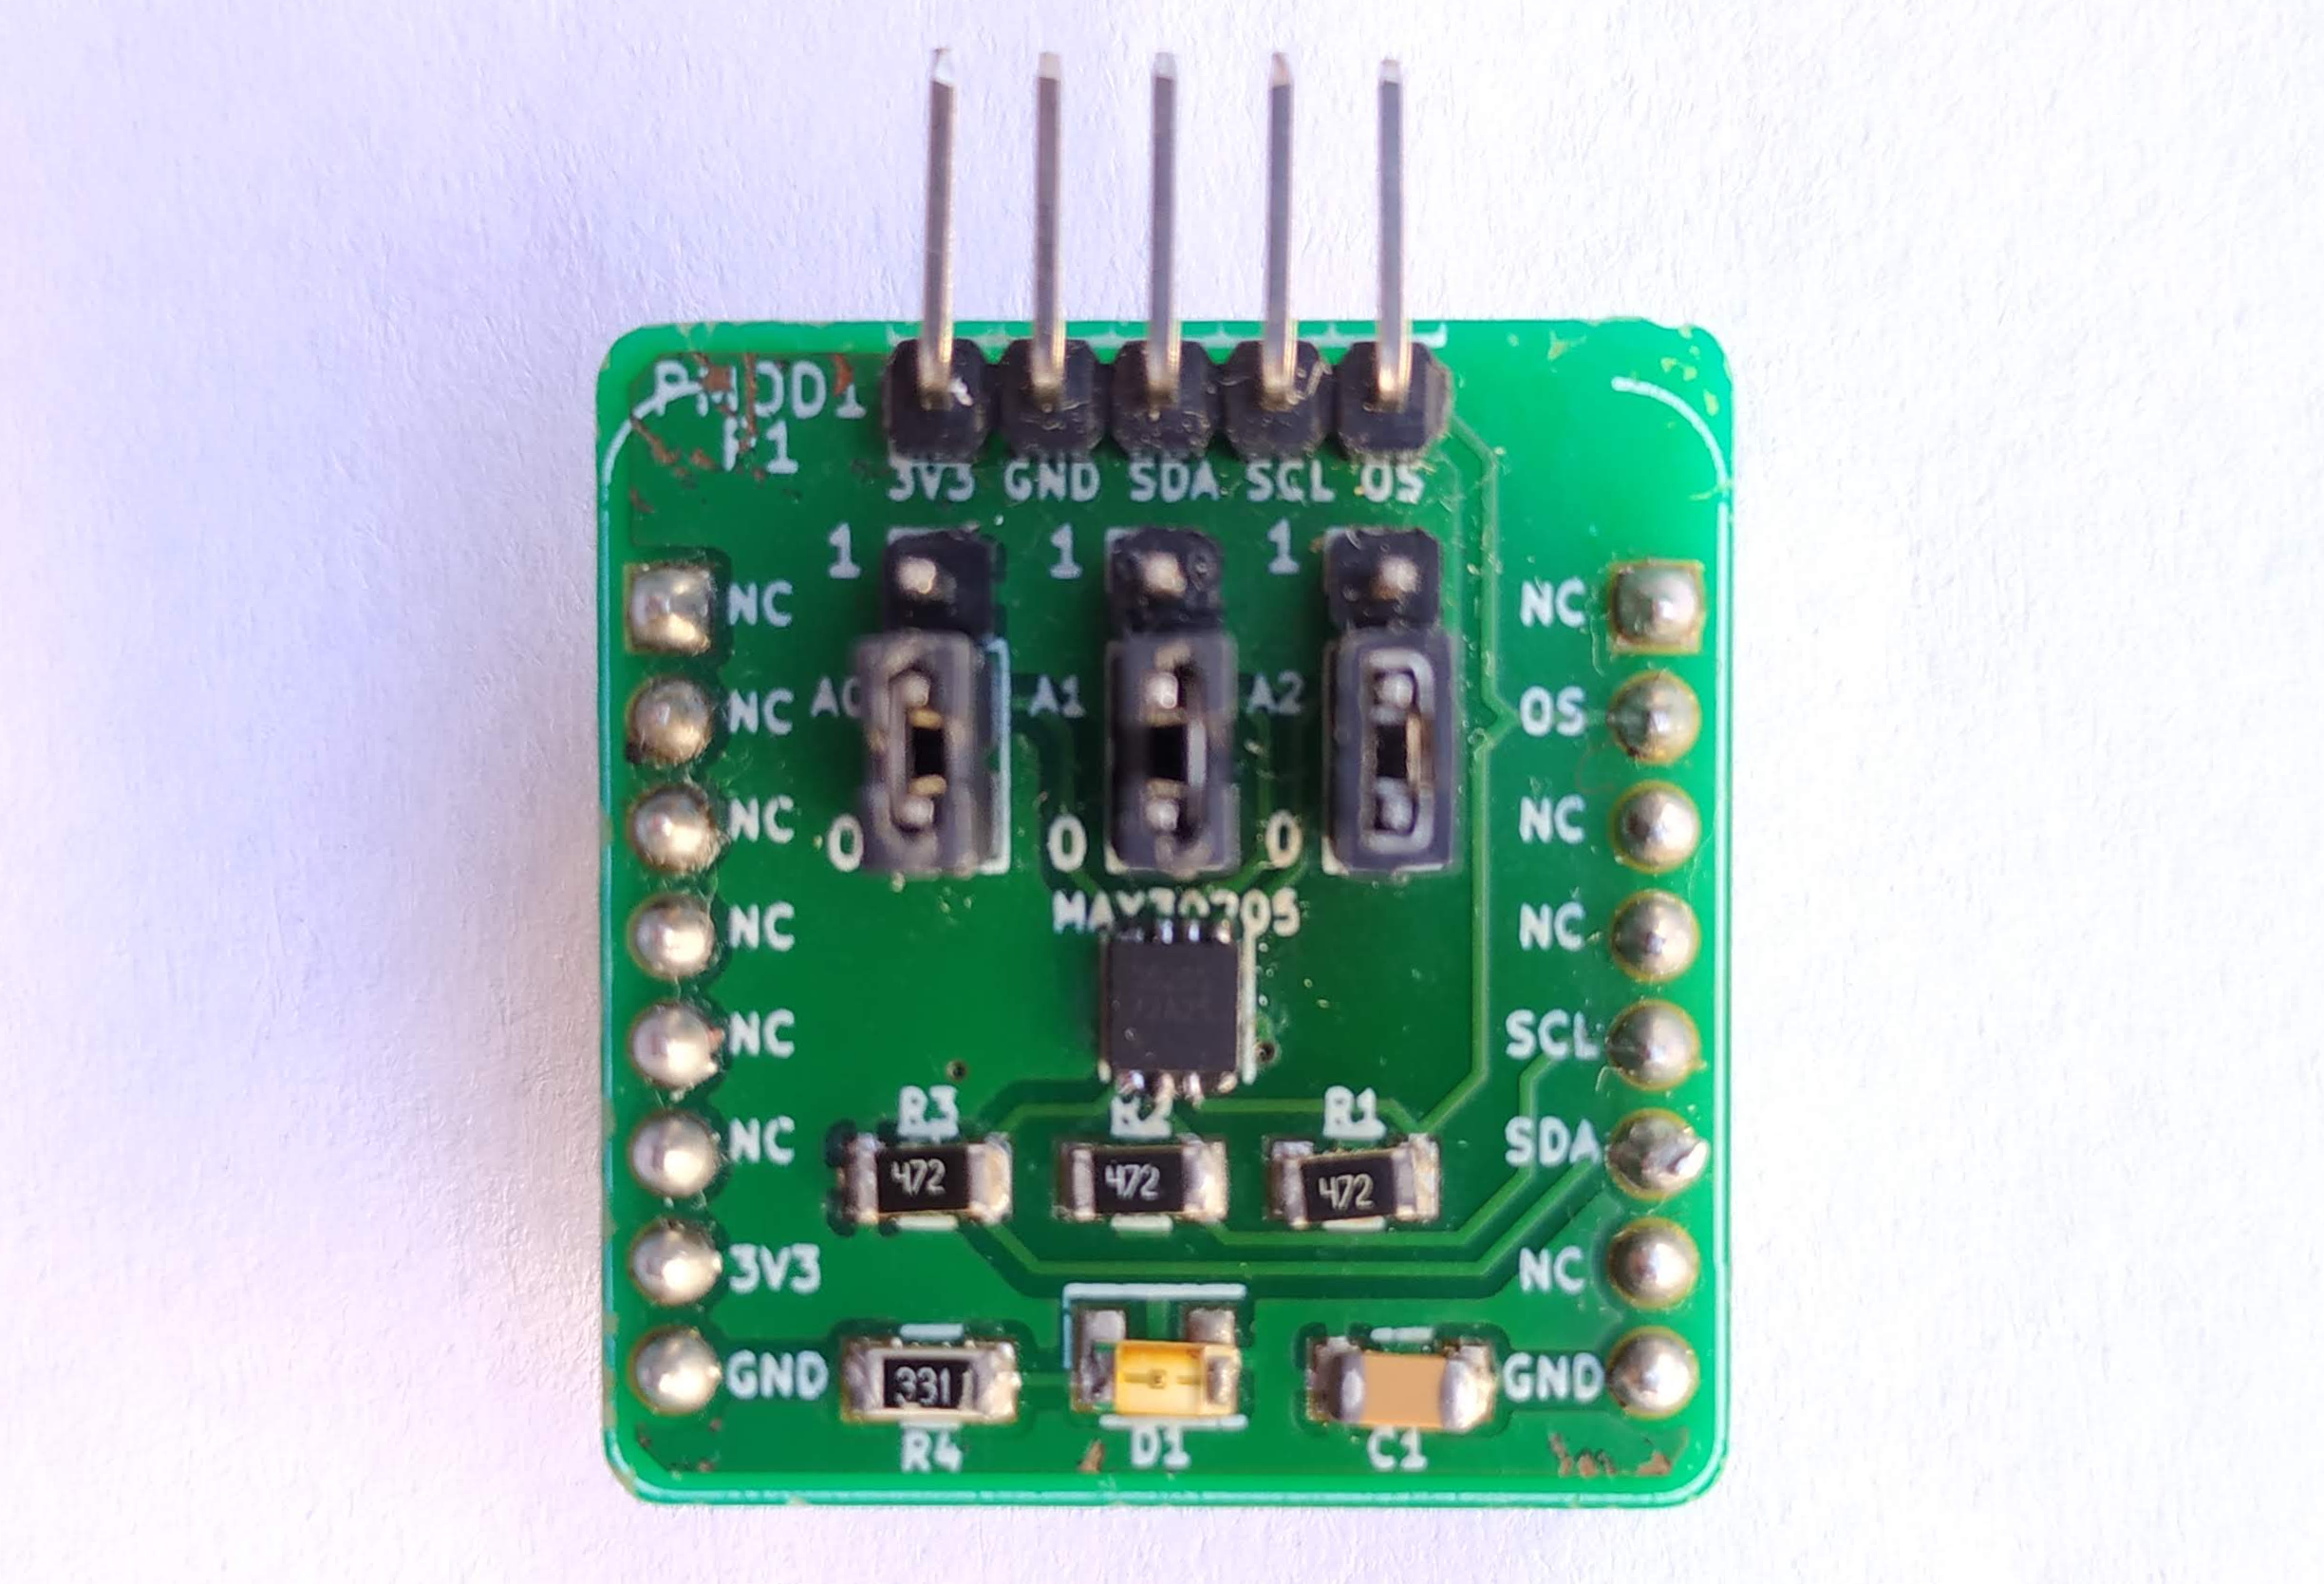
\includegraphics[width=0.6\textwidth]{Analisis/imagenes/MAX30205.jpg}}
%			\caption{MAX30205}
%			\label{fig:AnalisisMax30205}
%		\end{figure}
%	\clearpage
